\section{Wachstum}
\subsection{Langfristiger Wachstumstrend}
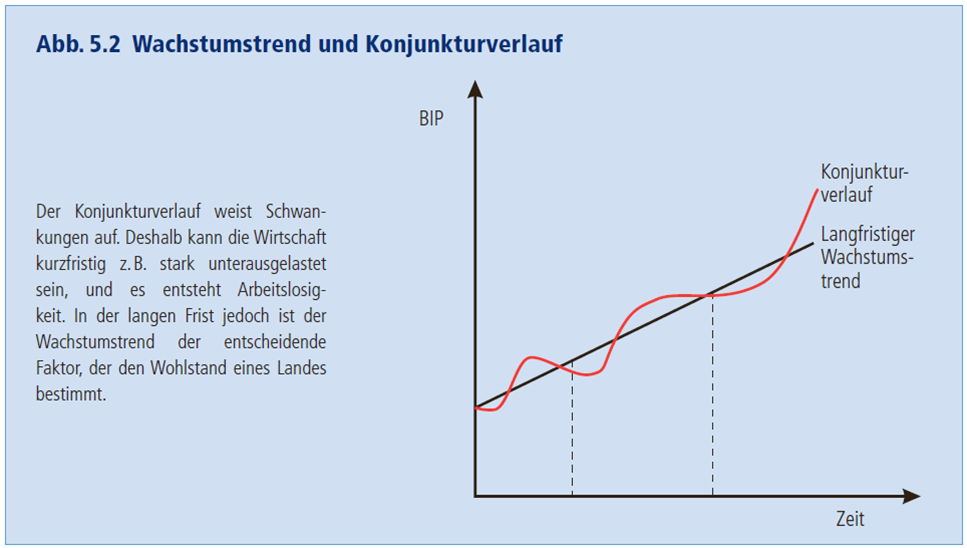
\includegraphics[width=0.65\linewidth]{images/wachstum.png}
\subsection{Quellen des Wachstums}
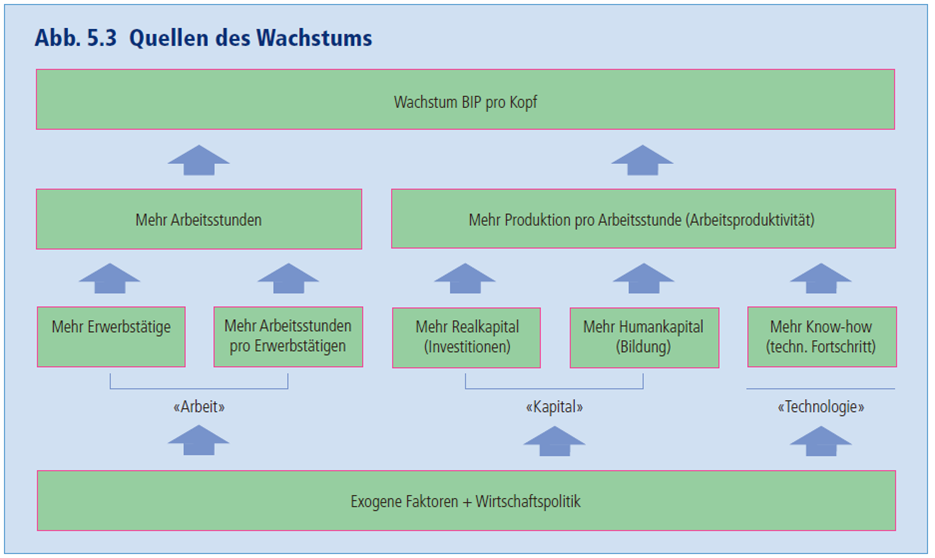
\includegraphics[width=0.65\linewidth]{images/quellen.png}
\subsubsection{Exogene Faktoren}
\begin{itemize}
	\item Ausstattung mir Rohstoffen
	\item Klima
	\item Nähe zu Handelspartnern
	\item Sozialkapital
	\subitem politische Stabilität
	\subitem Ausgestaltung der politischen Rechte
	\subitem Vertrauen in Eigentums- und Vertragsrechte
	\subitem tiefe Korruption
\end{itemize}
\begin{multicols}{2}
\subsubsection{Schweizer Wachstumssflaute}
\begin{itemize}
	\item Problem der Schweizer Hochpreisinsel (Abschottung Binnenmarkt)
	\item Höheres Wachstum der Schweizer Staatsquote
	\item Nicht schuld ist die höhere Immigration
\end{itemize}
\subsubsection{Staatsquote}
\begin{itemize}
	\item Staatsquote = (öffentliche Konsum + öffentliche Investitionen) / nominales BIP
	\item Zunehmender staatsnaher Sektor (Erziehung, Gesundheit, Soziale und Energie) expandiert und wirkt als Bremse für das Wachstum
\end{itemize}
\end{multicols}